\documentclass{tufte-handout}

%\geometry{showframe}% for debugging purposes -- displays the margins

\usepackage{amsmath}

% Set up the images/graphics package
\usepackage{asymptote} % for asymptote graphics
\usepackage{graphicx}
\setkeys{Gin}{width=\linewidth,totalheight=\textheight,keepaspectratio}
\graphicspath{{graphics/}}

\title{Summing Approximations}
\author[Warren MacEvoy]{Warren MacEvoy}
% \date{24 January 2009}  % if the \date{} command is left out, the current date will be used

% The following package makes prettier tables.  We're all about the bling!
\usepackage{booktabs}

\hypersetup{colorlinks} % Comment this line if you don't wish to have colored links
\usepackage{amsmath}
\usepackage{amssymb}
\usepackage{amsthm}
\usepackage{listings}
\usepackage{siunitx} % align decimals in tables
\usepackage{nth}     % 1st, 2nd, ...
\usepackage{microtype} % Improves character and word spacing
\usepackage{asymptote} % for asymptote graphics
\usepackage{ccicons}
\usepackage{lipsum} % Inserts dummy text
\usepackage{booktabs} % Better horizontal rules in tables
\usepackage{graphicx} % Needed to insert images into the document

% The units package provides nice, non-stacked fractions and better spacing
% for units.
\usepackage{units}

% The fancyvrb package lets us customize the formatting of verbatim
% environments.  We use a slightly smaller font.
\usepackage{fancyvrb}
\fvset{fontsize=\normalsize}

% Small sections of multiple columns
\usepackage{multicol}

% Provides paragraphs of dummy text
\usepackage{lipsum}

% These commands are used to pretty-print LaTeX commands
\newcommand{\doccmd}[1]{\texttt{\textbackslash#1}}% command name -- adds backslash automatically
\newcommand{\docopt}[1]{\ensuremath{\langle}\textrm{\textit{#1}}\ensuremath{\rangle}}% optional command argument
\newcommand{\docarg}[1]{\textrm{\textit{#1}}}% (required) command argument
\newenvironment{docspec}{\begin{quote}\noindent}{\end{quote}}% command specification environment
\newcommand{\docenv}[1]{\textsf{#1}}% environment name
\newcommand{\docpkg}[1]{\texttt{#1}}% package name
\newcommand{\doccls}[1]{\texttt{#1}}% document class name
\newcommand{\docclsopt}[1]{\texttt{#1}}% document class option name

\theoremstyle{definition}
\newtheorem{definition}{Definition}
\theoremstyle{example}
\newtheorem{example}{Example}
\theoremstyle{theorem}
\newtheorem{theorem}{Theorem}
\begin{document}

\maketitle% this prints the handout title, author, and date

\begin{abstract}
\noindent Understanding asymptotic behavior of a series or function is useful.
\end{abstract}

%\printclassoptions

\section{Estimating Sums}

\begin{figure}
\begin{center}
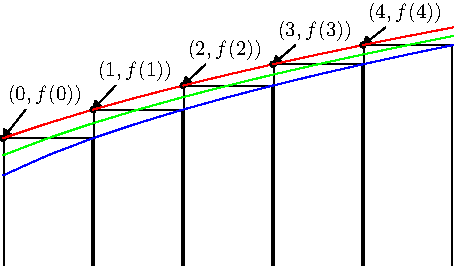
\includegraphics[width=1.00\linewidth]{graphics/intsum.pdf}
\end{center}
\caption{\label{fig:intmid}Comparing sum (black rectangles) with integrals of increasing $f$ (red), $f$ shifted -1/2 (green), and $f$ shifted -1 (blue).}
\label{fig:intmid}
\end{figure}

Summing is a linear operation, so

\begin{equation}
  \sum_{k=0}^{n-1} \left[ \alpha f(k) + \beta g(k) \right] = \alpha \sum_{k=0}^{n-1} f(k) + \beta \sum_{k=0}^{n-1} g(k) \,.
\end{equation}

Summing powers of $k$:

\begin{equation}
  \sum_{k=0}^{n-1} 1 = n \,.
\end{equation}

\begin{equation}
  \sum_{k=0}^{n-1} k = \frac{1}{2} n(n-1) = \frac{1}{2} n^2 + O(n)\,.
\end{equation}

\begin{equation}
  \sum_{k=0}^{n-1} k^2 = \frac{1}{3}n(n-1/2)(n-1) = \frac{1}{3} n^3 + O(n^2) \,.
\end{equation}

\begin{equation}
  \sum_{k=0}^{n-1} k^3 = \frac{1}{4}n^2(n-1)^2 = \frac{1}{4} n^4 + O(n^3) \,.
\end{equation}

Generally, for $p>0$,

\begin{equation}
  \sum_{k=0}^{n-1} k^p \approx \frac{1}{p+1} (n-1/2)^{p+1} = \frac{1}{p+1} n^{p+1} +O(n^p) \,.
\end{equation}

Estimating sums with integrals.

If $f(x)$ is increasing, then
\begin{equation}
\int_{a-1}^{b} f(x) \, dx \leq \sum_{k=a}^{b} f(k) \approx \int_{a-1/2}^{b+1/2} f(x) dx \leq \int_{a}^{b+1} f(x) \, dx
\end{equation}

\end{document}
